\documentclass[12pt]{article}
\usepackage[utf8]{inputenc}
\usepackage{graphicx} % Allows you to insert figures
\usepackage{amsmath} % Allows you to do equations
\usepackage{fancyhdr} % Formats the header
\usepackage{geometry} % Formats the paper size, orientation, and margins
\linespread{1.25} % about 1.5 spacing in Word
\setlength{\parindent}{0pt} % no paragraph indents
\setlength{\parskip}{1em} % paragraphs separated by one line
\usepackage[format=plain,
            font=it]{caption} % Italicizes figure captions
\usepackage[english]{babel}
\usepackage{csquotes}
\usepackage{minted}
\renewcommand{\headrulewidth}{0pt}
\geometry{letterpaper, portrait, margin=1in}
\setlength{\headheight}{14.49998pt}

\newcommand\titleofdoc{\Large{\textbf{EE2703 - Applied Programming Language\\End Semester Exam}}}
\newcommand\GroupName{EE20B136}

\begin{document}
\begin{titlepage}
   \begin{center}
        \vspace*{4cm} % Adjust spacings to ensure the title page is generally filled with text

        \Huge{\titleofdoc} 

        \vspace{3 cm}
        \Large{Syam SriBalaji T}
       
        \vspace{0.25cm}
        \large{EE20B136}
       
        \vspace{3 cm}
        \Large{May 12, 2022}
        
        \vspace{0.25 cm}
        \Large{EE2703: Jan-May 2022}
       

       \vfill
    \end{center}
\end{titlepage}

\setcounter{page}{2}
\pagestyle{fancy}
\fancyhf{}
\rhead{\thepage}


\newpage
\section*{\textbf{Contents:}}

\begin{itemize}
  \item Current distribution in a dipole antenna
  \item Finding $P_{ij}$ , $P_{B}$ (Coefficient matrix of Magnetic vector potential $\overrightarrow{A}_{z,i}$)
  \item Finding $Q_{ij}$ , $Q_{B}$ (Coefficients matrix of Magnetic field $\overrightarrow{H}_{\phi}(r,z_{i})$)
  \item Finding Current through Magnetic vector potential method
  \item Comparison of I vs. z in different methods and variable N
\end{itemize}

\section*{Dipole Antenna: }
It consists of two conductive element i.e., rods or wires and a feeder(connecting the rods). This wire or rod are separated into two sections by an insulator. The radio-frequency (RF) voltage source is applied to the center between the two sections of the dipole antenna. The length of the metal wires is approximately half of the maximum wavelength (i.e.,= $\frac{\lambda}{2}$) of the current passing through it in free space at the frequency of operation. 

The current is maximum and voltage is minimum at the center. Conversely, the current is minimum and voltage is maximum at the ends of the dipole antenna. It can either be used as transmitting or receiving antenna. And it is widely used in radio and telecommunications.\\\\


\begin{figure}[h!]
\centering
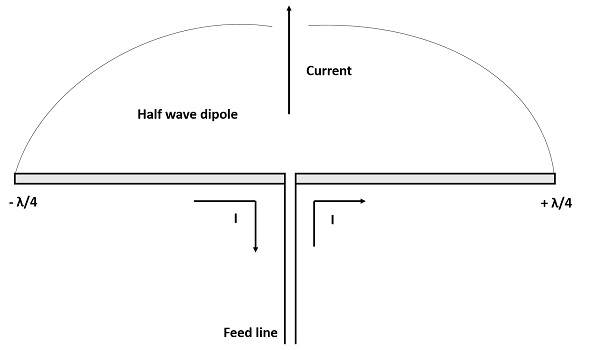
\includegraphics[height=7cm]{Dipole1.jpg}
\label{fig:exemplo}
\end{figure}

\newpage
\section*{Current through antenna: }

From the standard analysis, we assume the current in the antennas to be-
  \begin{equation}
    I=
    \begin{cases}
      Im\times sin(k(l-z)) &  0 \le z \le l \\
      Im\times sin(k(l+z))  &  −l \le z \lt< 0 
    \end{cases}
  \end{equation}
where,\\
Im=current injected to the antenna\\
k=wave number=$\frac{2\pi}{\lambda}$ \\
l=quarter wavelength=$\frac{\lambda}{4}$ \\
z=distance from reference point along the rod

By this way, we get a set of values for the current through the antenna(for N=4), which is-
\begin{gather*}
    I
    =
    \begin{pmatrix}
    0.0\\
    0.3827\\
    0.7071\\
    0.9239\\
    1.0\\
    0.9239\\
    0.7071\\
    0.3827\\
    0.0\\
    \end{pmatrix}
\end{gather*}
We can clearly see the sinusoidal nature of the current, and we can observe the maximum current in the middle and current minimum current at the ends of the rod.

\textbf{\textit{Pseudo code: 1}} \\
$I=Im\times sin(k(l\pm z))$ \\
for $0 \le z \le l \rightarrow +$\\
for $−l \le z \lt< 0 \rightarrow -$

\newpage
\section*{Ampere’s Circuital law: }
Around every closed curve, the line integral of the magnetic field B is equal to  $\mu _{o}$ times the net current I threading through the region contained by the curve.

\begin{equation}
  \oint H’.dl’=\sum I 
\end{equation}

Applying the same in dipole antenna where $radius=a$, we get-
\begin{equation}
   2\pi a H_{\phi}(z_{i}) = I_{i} 
\end{equation}

We convert the same into matrix equation, we get-

\[ \begin{pmatrix}
    H_{\phi}(z_1) \\
    \dots \\
    H_{\phi}(z_{N-1}) \\
    H_{\phi}(z_{N+1}) \\
    \dots \\
    H_{\phi}(z_{2N-1} 
\end{pmatrix}
= \frac{1}{2\pi a} \begin{pmatrix} 
    1 & \dots & 0 & 0 & \dots & 0 \\
    \dots & \dots & \dots & \dots & \dots & \dots \\
    0 & \dots & 1 & 0 & \dots & 0 \\
    0 & \dots & 0 & 1 & \dots & 0 \\
    \dots & \dots & \dots & \dots & \dots & \dots \\
    0 & \dots & 0 & 0 & \dots & 1 \\
\end{pmatrix}\begin{pmatrix}
    J_1 \\ \dots \\ J_{N-1} \\ J_{N+1} \\ \dots \\ J_{2N-1}
\end{pmatrix} \\
= M \times J
\]
\\\\
\textbf{\textit{Pseudo code: 2}} \\
Create matrix J, order=$[2N-2 \times 1]$, initially define with zeros$\\
$Create matrix M $=\frac{1}{2 \pi a} \times$ identity matrix of order [2N-2,2N-2]$

\newpage
\section*{Calculating Magnetic vector potential:}

Firstly, we will be calculating Magnetic vector potential $\overrightarrow{A}_{z,i}$
\[A_{z,i} = \sum_{j} I_j\left(\frac{\mu_{o}}{4\pi} \times \frac {exp(-jk R_{ij})dz'j}{R{ij}}\right)\]

Writing it in matrix form, we get-
\[A_z,j = \sum{j} P_{ij} I_j + P_B I_N \]

From the above equation we write the $P_B$ and $P_{ij}$ as,

\[P_B =  \frac{\mu_{o}}{4\pi} \times \frac {exp(-jk R_{iN}) \times dz'_j}{R_{iN}}\]
\[P_{ij} =  \frac{\mu_{o}}{4\pi} \times \frac {exp(-jk R_{ij}) \times dz'_j}{R_{ij}}\]
where, \[ R_{ij} = \sqrt{a^2 + (z_i - z_j)^2} \]

Solving for N=4, we get-

\begin{gather*}
    R_{ij}
    =
    \begin{pmatrix}
    0.01& 0.13& 0.25& 0.5 & 0.63& 0.75\\
    0.13& 0.01& 0.13& 0.38& 0.5 & 0.63\\
    0.25& 0.13& 0.01& 0.25& 0.38& 0.5 \\
    0.5 & 0.38& 0.25& 0.01& 0.13& 0.25\\
    0.63& 0.5 & 0.38& 0.13& 0.01& 0.13\\
    0.75& 0.63& 0.5 & 0.25& 0.13& 0.01\\
    \end{pmatrix}
\end{gather*}

\begin{gather*}
    P_{B}
    =
    \begin{pmatrix}
    1.27e-08-3.08e-08j\\
    3.53e-08-3.53e-08j\\
    9.20e-08-3.83e-08j\\
    9.20e-08-3.83e-08j\\
    3.53e-08-3.53e-08j\\
    1.27e-08-3.08e-08j\\
    \end{pmatrix}
\end{gather*}

\newpage
\newgeometry{left=0.8cm,bottom=0.1cm}
\begin{gather*}
    P_{ij}
    =
    \left(\begin{smallmatrix}
     1.25e-06-3.93e-08j&  9.20e-08-3.83e-08j&  3.53e-08-3.53e-08j&-7.85e-12-2.50e-08j& -7.66e-09-1.85e-08j& -1.18e-08-1.18e-08j\\
     9.20e-08-3.83e-08j&  1.25e-06-3.93e-08j&  9.20e-08-3.83e-08j& 1.27e-08-3.08e-08j& -7.85e-12-2.50e-08j& -7.66e-09-1.85e-08j\\
     3.53e-08-3.53e-08j&  9.20e-08-3.83e-08j&  1.25e-06-3.93e-08j& 3.53e-08-3.53e-08j&  1.27e-08-3.08e-08j& -7.85e-12-2.50e-08j\\
    -7.85e-12-2.50e-08j&  1.27e-08-3.08e-08j&  3.53e-08-3.53e-08j& 1.25e-06-3.93e-08j&  9.20e-08-3.83e-08j&  3.53e-08-3.53e-08j\\
    -7.66e-09-1.85e-08j& -7.85e-12-2.50e-08j&  1.27e-08-3.08e-08j& 9.20e-08-3.83e-08j&  1.25e-06-3.93e-08j&  9.20e-08-3.83e-08j\\
    -1.18e-08-1.18e-08j& -7.66e-09-1.85e-08j& -7.85e-12-2.50e-08j& 3.53e-08-3.53e-08j&  9.20e-08-3.83e-08j&  1.25e-06-3.93e-08j\\
    \end{smallmatrix}\right)
\end{gather*}\\\\

\textbf{\textit{Pseudo code: 3}}\\
for $0 \le i,j \le 2N$\\
Use this, $R_{ij} = \sqrt{a^2 + (z_i - z_j)^2}$\\
$P_{ij} =  \frac{\mu_{o}}{4\pi} \times \frac {exp(-jk R_{ij}) \times dz'_j}{R_{ij}}$\\
find matrix $R_{ij}, order=[2N-2,2N-2], \implies$ ignore all sides and middle cross rows and columns \\
find matrix $R_{iN}, order=[2N-2,1], \implies$ ignore first, middle and last elements\\
find matrix $P_{ij}, order=[2N-2,2N-2], \implies$ ignore all sides and middle cross rows and columns\\
find matrix $P_{B}, order=[2N-2,1], \implies$ ignore first, middle and last elements\\

\restoregeometry



\newpage
\section*{Calculating Magnetic field vector:}
Secondly lets calculate Magnetic field vector $\overrightarrow{H}_{\phi}(r,z_{i})$)-
\[H_{\phi}(r,z) = -\frac{1}{\mu}\frac{\partial A_z}{\partial r}\]


Now, let's expand this and convert it into matrix form and solve further-

\[H_\phi(r,Z_i) = \sum P_{ij} \times \frac{a}{\mu0} ( \frac{jk}{R_{ij}} +\frac{1}{R_{ij}^2})I_j
+P_B \frac{a}{\mu0} (\frac{jk}{R_{iN}} +\frac{1}{R_{iN}^2})I_m\]

\[H_{\phi}(r,z_i) = \sum Q_i_j I_j + Q_B_i I_m\]

From the above equation, we can write $Q_B$ and $Q_{ij}$-

\[Q_{ij}=P_i_j \times \frac{a}{\mu_{o}} ( \frac{jk}{R_{ij}} +\frac{1}{R_{ij}^2})\]

\[Q_B =P_B \times \frac{a}{\mu_{o}} (\frac{jk}{R_{iN}} +\frac{1}{R_{iN}^2})\]

Solving for N=4, we get-
\begin{gather*}
    Q_{B}
    =
    \begin{pmatrix}
    0.0028-0.0009j\\
    0.008 -0.001j \\
    0.0542-0.001j \\
    0.0542-0.001j \\
    0.008 -0.001j \\
    0.0028-0.0009j\\
    \end{pmatrix}
\end{gather*}

\newpage

\newgeometry{left=1cm,bottom=0.1cm}
\begin{gather*}
    Q_{ij}
    =
    \left(\begin{smallmatrix}
    9.9521e+01-0.001j & 5.4208e-02-0.001j & 8.0201e-03-0.001j & 1.2493e-03-0.0008j& 5.8288e-04-0.0007j& 2.2597e-04-0.0006j\\
    5.4208e-02-0.001j & 9.9521e+01-0.001j & 5.4208e-02-0.001j & 2.7723e-03-0.0009j& 1.2493e-03-0.0008j& 5.8288e-04-0.0007j\\
    8.0201e-03-0.001j & 5.4208e-02-0.001j & 9.9521e+01-0.001j & 8.0201e-03-0.001j & 2.7723e-03-0.0009j& 1.2493e-03-0.0008j\\
    1.2493e-03-0.0008j& 2.7723e-03-0.0009j& 8.0201e-03-0.001j & 9.9521e+01-0.001j & 5.4208e-02-0.001j & 8.0201e-03-0.001j \\
    5.8288e-04-0.0007j& 1.2493e-03-0.0008j& 2.7723e-03-0.0009j& 5.4208e-02-0.001j & 9.9521e+01-0.001j & 5.4208e-02-0.001j \\
    2.2597e-04-0.0006j& 5.8288e-04-0.0007j& 1.2493e-03-0.0008j& 8.0201e-03-0.001j & 5.4208e-02-0.001j & 9.9521e+01-0.001j \\
    \end{smallmatrix}\right)
\end{gather*}

\\\\
\textbf{\textit{Pseudo code: 4}}\\
for $0 \le i,j \le 2N$\\
From this common formula, $Q_{ij}=P_i_j \times \frac{a}{\mu_{o}} ( \frac{jk}{R_{ij}} +\frac{1}{R_{ij}^2})$\\
find matrix $Q_{ij}, order=[2N-2,2N-2],\implies$ ignore all sides and middle cross rows and columns \\ 
find matrix $Q_{B}, order=[2N-2,1], \implies$ ignore first, middle and last elements\\

\restoregeometry

\newpage
\section*{Comparison of current plots:}

For N=4,
\begin{figure}[h!]
\centering
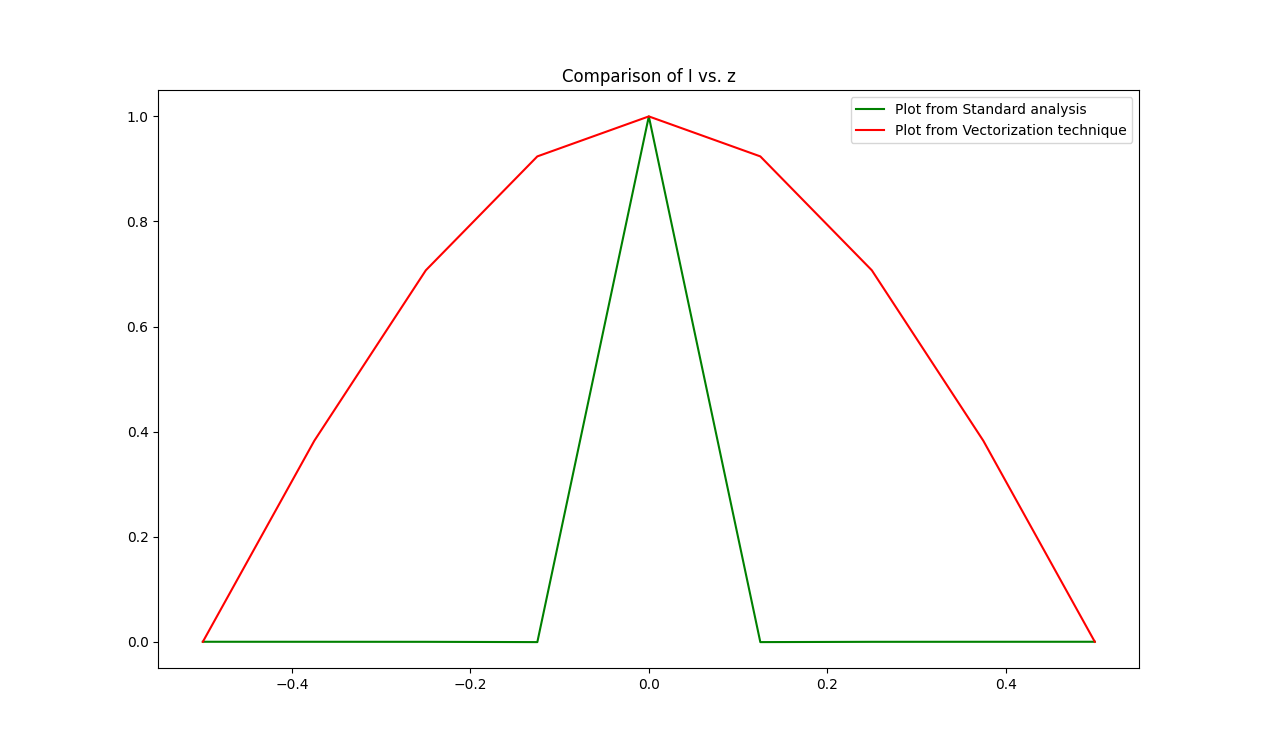
\includegraphics[height=6.5cm]{N4.png}
\label{fig:exemplo}
\end{figure}

Here we can see a large deviation from the actual current distribution, it is because number of divisions along the length which we take is very small.

For N=100,
\begin{figure}[h!]
\centering
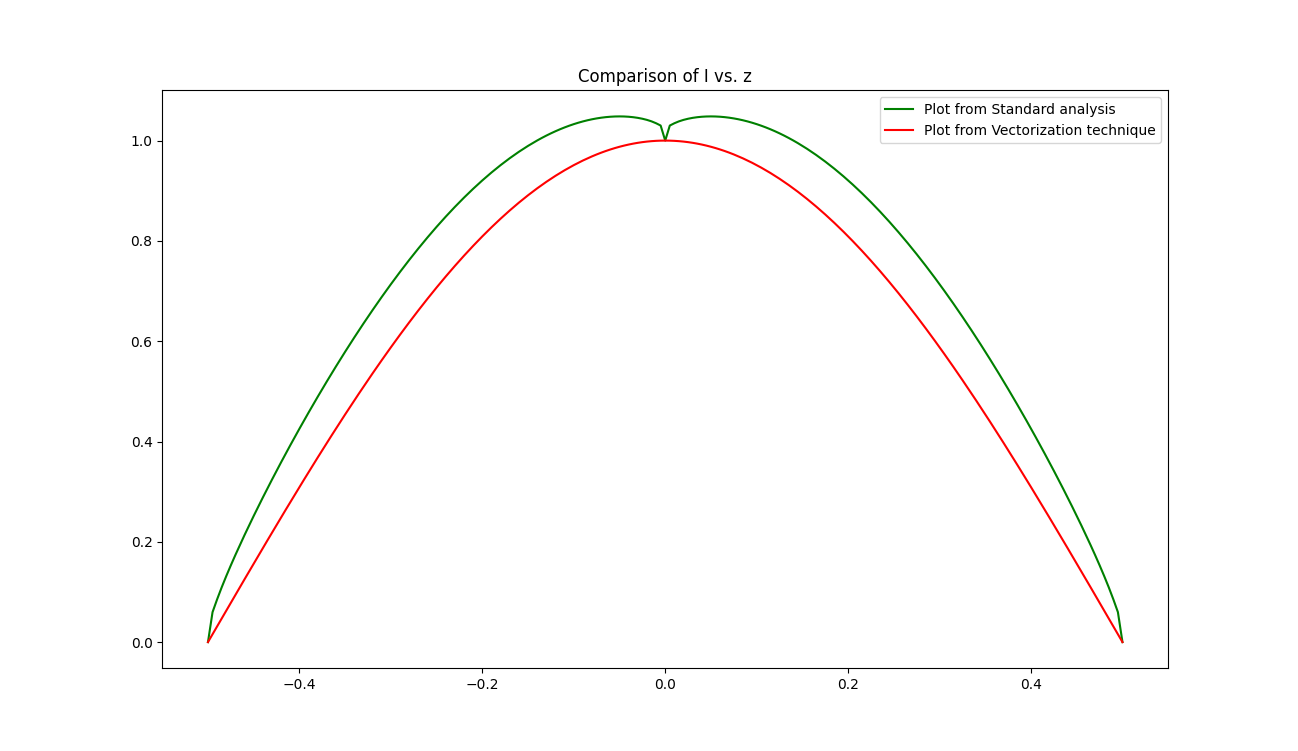
\includegraphics[height=6.5cm]{N100.png}
\label{fig:exemplo}
\end{figure}

Here relatively we can see very less deviation from the actual graph. And also we can see a abnormal dip in the middle of the rod or wire. It is caused because the vectorisation method which we did is just a good approximation from the boundary conditions we had, but not a accurate one. 

\newpage
\textbf{\textit{Pseudo code: 5}}\\\\
From $(M - Q) \times J = Q_{B} \times I_{M}$ find J\\
Incorporate boundary conditions (add first, middle, last elements) to J and call it $J_final$\\
Plot (J\_final vs. z) and (I vs. z) for N=4 and 100


\section*{\textbf{Conclusion:}}
We analysed Current distribution in  a dipole antenna through two methods. And we even saw the comparison of plots between them too. On the way, we did dealt with lot of interesting matrices creation. Thus, Current in  half-wave dipole antenna varies sinusoidally along the length of the rod covering half wavelength.

\begin{center} 
\textbf{Thank you!}
\end{center} 
\end{document}
